%%%%%%%%%%%%%%%%%%%%%%%%%%%%%%%%%%%%%%%%%%%%%%%%%%%%%%%%%%%%%%%%%%%%%%%%%%%%%%%
%% Descr:       Vorlage für Berichte der DHBW-Karlsruhe
%% Author:      Prof. Dr. Jürgen Vollmer, vollmer@dhbw-karlsruhe.de
%% $Id: bericht.tex,v 1.19 2016/03/16 16:59:41 vollmer Exp $
%%  -*- coding: utf-8 -*-
%%%%%%%%%%%%%%%%%%%%%%%%%%%%%%%%%%%%%%%%%%%%%%%%%%%%%%%%%%%%%%%%%%%%%%%%%%%%%%%

\documentclass[
   ngerman          % neue deutsche Rechtschreibung
  ,a4paper          % Papiergrösse
% ,twoside          % Zweiseitiger Druck (rechts/links)
% ,10pt             % Schriftgrösse
  ,11pt
% ,12pt
  ,pdftex
%  ,disable         % Todo-Markierungen auschalten
]{report}

% Bitte die Codierung Ihrer Dateien auswählen:
% \usepackage[latin1]{inputenc}    % Für UNIX mit ISO-LATIN-codierten Dateien
% \usepackage[applemac]{inputenc}  % Für Apple Mac
% \usepackage[ansinew]{inputenc}   % Für Microsoft Windows
\usepackage[utf8]{inputenc}        % UTF-8 codierte Dateien
                                   % Dieses Dokument ist unter Unix erstellt, daher
                                   % wird diese Input-Codierung benutzt.

\usepackage{bericht}
\usepackage{multirow}

%%%%%%%%%%%%%%%%%%%%%%%%%%%%%%%%%%%%%%%%%%%%%%%%%%%%%%%%%%%%%%%%%%%%%%%%%%%%%%%
%% Angaben zur Arbeit
%%%%%%%%%%%%%%%%%%%%%%%%%%%%%%%%%%%%%%%%%%%%%%%%%%%%%%%%%%%%%%%%%%%%%%%%%%%%%%%

\newcommand{\Autor}{Pascal Stephan}
\newcommand{\MatrikelNummer}{3977689}
\newcommand{\Kursbezeichnung}{TINF18B4}

\newcommand{\FirmenName}{INIT SE}
\newcommand{\FirmenStadt}{Karlsruhe}
% \newcommand{\FirmenLogoDeckblatt}{\includegraphics[width=3cm]{TODO}}

% Falls es kein Firmenlogo gibt:
\newcommand{\FirmenLogoDeckblatt}{}

\newcommand{\BetreuerFirma}{}
\newcommand{\BetreuerDHBW}{Mirko Dostmann}

%%%%%%%%%%%%%%%%%%%%%%%%%%%%%%%%%%%%%%%%%%%%%%%%%%%%%%%%%%%%%%%%%%%%%%%%%%%%%%%%%%%%%

\newcommand{\Was}{Technische Dokumentation} 
% Wird auf dem Deckblatt in der Erklärung benutzt

%%%%%%%%%%%%%%%%%%%%%%%%%%%%%%%%%%%%%%%%%%%%%%%%%%%%%%%%%%%%%%%%%%%%%%%%%%%%%%%%%%%%%

\newcommand{\Titel}{Programmentwurf}
\newcommand{\AbgabeDatum}{31.05.2021}

\newcommand{\Dauer}{5. + 6. Semester}

%\newcommand{\Abschluss}{Bachelor of Engineering}
\newcommand{\Abschluss}{Advanced Software Engineering}

%\newcommand{\Studiengang}{Informationstechnik}
\newcommand{\Studiengang}{Angewandte Informatik}

\hypersetup{%%
  pdfauthor={\Autor},
  pdftitle={\Titel},
  pdfsubject={\Was}
}

%%%%%%%%%%%%%%%%%%%%%%%%%%%%%%%%%%%%%%%%%%%%%%%%%%%%%%%%%%%%%%%%%%%%%%%%%%%%%%%

% Wenn \includeonly{..} benutzt wird, werden nur diese Kaptitel ausgegeben.
\includeonly{
  abk
  ,0_einleitung
  ,1_kapitel
  ,2_kapitel
  ,3_kapitel
  ,4_kapitel
  ,5_kapitel
  ,6_kapitel
  ,7_kapitel
  ,8_kapitel
}

%%%%%%%%%%%%%%%%%%%%%%%%%%%%%%%%%%%%%%%%%%%%%%%%%%%%%%%%%%%%%%%%%%%%%%%%%%%%%%%

% Benutzt man das "biblatex"-Paket, dann muß das hier stehen:
% siehe auch die mit BIBLATEX markierten Zeilen in bericht.sty
\bibliography{bericht}
\newcounter{savepage}
\begin{document}

%%%%%%%%%%%%%%%%%%%%%%%%%%%%%%%%%%%%%%%%%%%%%%%%%%%%%%%%%%%%%%%%%%%%%%%%%%%%%%%

\pagenumbering{roman}
\begin{titlepage}
  \begin{center}
    \vspace*{-2cm}
    \FirmenLogoDeckblatt\hfill
\includegraphics[width=4cm]{dhbw-logo}\\[2cm]
    {\Huge \Titel}\\[2cm]
    {\Huge\scshape \Was}\\[2cm]
    {\large für die Vorlesung}\\[0.5cm]
    {\Large \Abschluss}\\[0.5cm]
    {\large des Studienganges \Studiengang}\\[0.5cm]
    {\large an der}\\[0.5cm]
    {\large Dualen Hochschule Baden-Württemberg Karlsruhe}\\[0.5cm]
    {\large von}\\[0.5cm]
    {\large\bfseries \Autor}\\[1cm]
    {\large Abgabedatum \AbgabeDatum}
    \vfill
  \end{center}
  \begin{tabular}{l@{\hspace{2cm}}l}
    Bearbeitungszeitraum          & \Dauer           \\
    Matrikelnummer                & \MatrikelNummer  \\
    Kurs                          & \Kursbezeichnung \\
    Gutachter der Studienakademie & \BetreuerDHBW    \\
  \end{tabular}
\end{titlepage}

%%%%%%%%%%%%%%%%%%%%%%%%%%%%%%%%%%%%%%%%%%%%%%%%%%%%%%%%%%%%%%%%%%%%%%%%%%%%%%%

% Nur für Bachelorarbeiten einfügen:
\newpage
\tableofcontents           % Inhaltsverzeichnis hier ausgeben
\listoffigures             % Liste der Abbildungen
%\listoftables              % Liste der Tabellen
%%\lstlistoflistings         % Liste der Listings
%\listofequations           % Liste der Formeln

% Jetzt kommt der "eigentliche" Text
%%29 mtime=1458130901.64846426
30 atime=1458130911.887391657
29 ctime=1458130901.64846426
              % Abkürzungsverzeichnis
\setcounter{savepage}{\arabic{page}}
\pagenumbering{arabic}
\chapter{Einleitung}
In diesem Programmentwurf wurde Finanz/Banking-Anwendung entwickelt. Das projekt besteht aus einem backend und einem Frontend. Für das Backend wurde eine .NET Core WebApi 
erstellt und für das Frontend ein einfacher Client mit Hilfe von Windows Forms. Der Client dient dazu die Funktionen der API auszuführen und darzustellen. Die WebApi 
greift auf Anfrage des Clients auf eine InMemory-Datenbank zu und führt auf dieser Operationen aus. Da es sich hier um eine InMemory-Datenbank handelt, die im Speicher der Api läuft, 
wird die Datenbank resettet, wenn die WebApi gestoppt wird. 
\newline Das Frontend und das Backend wurden mit der Visual Studio 2019 Community Edition erstellt.
\newline Um das Testen der WebApi durch den Client zu vereinfachen, wird bei Start des Clients automatisch ein Test-Benutzer angelegt. Die Anmeldedaten für diesen Testnutzer sind:
\begin{itemize}
    \item Email: Test@test.com
    \item Passwort: Passw0rd
\end{itemize}
Dieser Benutzer wird als Admin angelegt und kann somit alle Funktionen der Anwendung nutzen. Welche Funktionen nicht genutzt werden können, wird später erklärt.
\newline Weiterhin werden bei Start 3 Banken auf der Datenbank angelegt, um Konten anlegen zu können, ohne dass eine Bank ausgewählt werden muss.
\newline Zum eigentlichen Programmentwurf gehört nur die WebApi. Alle Vorgaben für den Programmentwurf wurden in dieser Api umgesetzt und nicht im Client-Projekt. 
Der Client hilft nur beim Testen der Funktionen der Api.
\newline Als Admin-Benutzer können im Client neue Banken angelegt werden, die daraufhin jedem anderen benutzer sichtbar sind. Diese Funktion ist nicht für Nicht-Admin-Benutzer 
verfügbar, da nicht alle Benutzer die Möglichkeit haben sollten, neue Banken einzutragen, da diese daraufhin in den Clients aller Benutzer erscheinen. So wird verhindert, dass 
normale Benutzer zu viele Banken eintragen, auf denen Konten angelegt werden können oder Dopplungen entstehen.. 
\section{Installation}
\subsection{Anforderungen}
Um die WebApi zu starten wird folgende Software benötigt:
\begin{itemize}
    \item .NET SDK 5.0
    \item Visual Studio 2019 oder Visual Studio Code
\end{itemize}
\subsection{Starten der Anwendung mit Visual Studio 2019}
Um die WebApi in Visual Studio 2019 zu starten, wird die gesamte Projektmappe mit Visual Studio geöffnet. Im Solution-Explorer sind daraufhin folgende Projekte zu sehen:
\begin{itemize}
    \item Programmentwurf\_BankingApi
    \item Programmentwurf\_Banking\_Client
    \item Programmentwurf\_Mock\_Tests
    \item Programmentwurf\_xUnit\_Tests
\end{itemize}
In \glqq Programmentwurf\_BankingApi \grqq befinden sich die einzelnen Projekte der WebApi. Durch Rechtsklick auf die Solution im Solution-Explorer kann unter \glqq Startprojekte festlegen \grqq 
ausgewählt werden, welche Projekte durch drücken von F5 gestartet werden sollen. Hier wird für das Projekt \glqq 0\_Plugin \grqq die Option \glqq Starten \grqq ausgewählt. Optional kann auch 
für das Projekt \glqq Programmentwurf\_Banking\_Client \grqq die Option \glqq Starten \grqq ausgewählt werden, um auch den Client direkt zu starten.
\subsection{Starten der Anwendung mit Visual Studio Code}
Um die WebApi in Visual Studio Code zu starten, muss das Projekt \glqq 0\_Plugin \grqq ausgeführt werden. Dafür wird in den Ordner \glqq Programmentwurf\_BankingApi \grqq navigiert und von dort in 
den Projektordner \glqq 0\_Plugin \grqq . Dort wird über die Terminal-Konsole folgende Befehle ausgeführt:
\begin{itemize}
    \item dotnet build
    \item dotnet run
\end{itemize}
Mit \glqq dotnet \grqq build wird versucht die Anwendung zu kompilieren. Dadurch werden auch alle NuGet-Pakete heruntergeladen, die für die Entwicklung des Porgramms genutzt wurden.
\newline Mit \glqq dotnet run \grqq wird daraufhin die Anwendung gestartet. Wird die Anwendung über Visual Studio Code gestartet, ist sie über den localhost mit Port 5001 erreichbar.
\subsection{Benutzen der Anwendung}
Die WebApi kann entweder durch Postman oder den dazugehörigen Client getestet werden. Im GitHub-Repository befindet sich eine postman-Collection die genutzt werden kann um die WebApi mit Postman zu testen.
\newline Bei Ausführen des Clients wird ein Login-Screen geöffnet. Von diesem aus kann entweder ein neuer Benutzer registriert werden oder es wird der Admin-Benutzer zum einloggen genutzt, dessen Anmeldedaten zuvor schon erwähnt wurden. 
Daraufhin öffnet sich der Home-Screen von dem aus alle Funktionen erreichbar sind. 
\newline Es muss beachtet werden, dass jedesmal wenn etwas erstellt oder hinzugefügt wird über den Client, der Aktualisierungs-Button geklickt werden muss, um die Daten im Client zu aktualisieren.
\chapter{Domain Driven Design}
\section{Ubiquitous Language}
In \ref{table} wird die Ubiquitous Language der Domäne analysiert.
\begin{table}[]
    \begin{tabular}{|l|l|}
    \hline
    \textbf{Wort} & \textbf{Bedeutung} \\ \hline
    User & Ein User stellt eine Person dar, die ihre Konten verwalten möchte \\ \hline
    Konto & Ein Konto stellt eine Einheit dar, auf der Geld gespeichert wird \\ \hline
    Transaktion & \begin{tabular}[c]{@{}l@{}}Eine Transaktion ist ein Auftrag, der von einem Konto ausgeht \\ oder dieses betrifft. \\ Dies stellt beispielsweise eine Überweisung dar\end{tabular} \\ \hline
    Bank & \begin{tabular}[c]{@{}l@{}}Eine Bank ist ein Institu, das Konten von Personen hält und für diese \\ Personen Transaktionen ausführt\end{tabular} \\ \hline
    Anmelden / Login & Ein bereits registrierter User meldet sich an einem System an \\ \hline
    Registrieren & Eine Person erstellt sich einen User in einem System \\ \hline
    Adresse & \begin{tabular}[c]{@{}l@{}}Durch eine Adresse kann eindeutig identifiziert werden, \\ wo sich in dieser Domäne eine Bank befindet oder ein User lebt\end{tabular} \\ \hline
    Kontostand ändern & \begin{tabular}[c]{@{}l@{}}Das Geld, das auf einem Konto gespeichert ist, \\ wird entweder erhöht oder verringert\end{tabular} \\ \hline
    überweisen & \begin{tabular}[c]{@{}l@{}}Beim Überweisen wird eine transaktion erstellt, \\ die Geld von einem Konto auf ein anderes\\ überträgt\end{tabular} \\ \hline
    \end{tabular}
    \label{table}
\end{table}
\section{Analyse und Begründung der verwendeten muster des DDD}
\subsection{Value Objects (VO)}
Value Objects oder auch Wertobjekte sind Objekte, die unveränderbar sind. Diese werden einmal erstellt und sind daraufhin nichtmehr änderbar, da sie spezielle Werte repräsentieren. Sie besitzen keine Methoden, da sie nur auf ihre Werte reduziert werden.
Soll der Wert eines Value Objects doch geändert werden, müssen diese neu erstellt werden. In diesem Programmentwurf wurden Value Objects zum einen für die Adresse einer Bank erstellt und zum anderen für die Informationen einer Transaktion. 
Die Adresse ist ein gutes Beispiel für ein Value Object, da sich die Adresse einer Bank später normalerweise nicht ändert, außer die komplette Bank zieht in ein anderes Gebäude um. Dies geschieht jedoch nicht so häufig, dass die 
Adresse änderbar sein muss. Auch die Informationen einer Transaktion sollten unveränderbar sein, damit immer nachvollzogen werden kann, welcher Betrag von welchem Konto auf welches Konto überwiesen wurde. 
\newline In \ref{valueObject} wird ein Ausschnitt aus dem Adressen Value Object gezeigt:
\begin{figure}[htbp]
    \centering
    \fbox{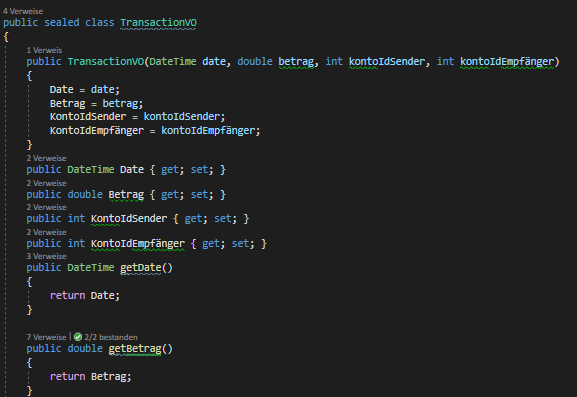
\includegraphics[width=10cm]{voAusschnitt.png}}
    \caption{\label{valueObject} AdressVO}
\end{figure}
\subsection{Entities}
Entities unterscheiden sich in den folgenden 3 Punkten von Value Objects:
\begin{itemize}
    \item Entities haben eine eindeutige Id
    \item Wenn Entities unterschiedliche Ids haben unterscheiden sie sich voneinander
    \item Eine Entity hat einen Lebenszyklus und verändert sich während diesem Zyklus häufiger
\end{itemize}
Es wurden in diesem Projekt folgende Entitäten angelegt:
\begin{itemize}
    \item User
    \item Konten
    \item Banken
\end{itemize}
Diese sind eindeutige Objekte die unterschieden werden müssen. Sie können sich von Zeit zu Zeit verändern. Vorallem Konten verändern sich häufig, da immer wieder Geld auf ein Konto 
eingezahlt und abgebucht wird. 
\newline Eine Entity sorgt auch dafür, dass keine ungültigen Werte gesetzt werden, um nicht in einen ungültigen zustand zu gelangen. Außerdem besitzen sie Methoden, die das Verhalten der 
Entitäten beschreiben.
\newline In \ref{kontoEntity} ist als Beispiel die erstellte KontoEntity zu sehen:
\begin{figure}[htbp]
    \centering
    \fbox{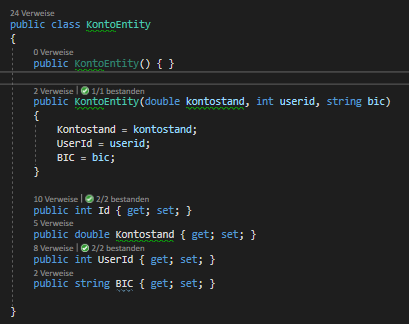
\includegraphics[width=10cm]{KontoEntity.png}}
    \caption{\label{kontoEntity} KontoEntity}
\end{figure}
\subsection{Aggregates}
Aggregate gruppieren Entities und Value Objects zu gemeinsam verwalteten Einheiten.
Aggregate helfen dabei die Komplexität der Beziehungen zwischen Objekten zu reduzieren. Die Entity im Aggregat dient als Aggregate Root Entity.
\newline Folgende Aggregate sind 
erstellt worden:
\begin{itemize}
    \item BankAggregate
    \item TransactionAggregate
\end{itemize}
Eine außenstehende Klasse muss eine Methode der Aggregate Root Entity aufrufen, sollte der innere Zustand geändert werden sollen. Dadurch wird sichergestellt, dass der Zustand immer den Domänenregeln entspricht.
\newline Das BankAggregate fasst die BankEntity und die dazugehörige Adresse zusammen. Das TransactionAggregate hält das Value Object 
für die Transaktioninfos und gibt jeder Transaktion eine Id. Hier könnte für die Transaktion noch eine TransactionEntity angelegt werden, diese würde allerdings nur die Id der Transaktion halten, weshalb sich dagegen entschieden wurde eine TransactionEntity zu erstellen. 
Weitere Informationen in der TransactionEntity zu halten macht keinen Sinn, da diese nicht änderbar sein sollen und deshalb in einem Value Object gehalten werden. Der Vollständigkeit halber sollte auch für die übrigen Entities wie UserEntity und KontoEntity ein Aggregat erstellt werden, die nur die jeweilige Entity besitzen. 
Darauf wurde jedoch verzichtet, um die Übersichtlichkeit des Projektes zu verbessern. Es kam öfters zu Verwirrungen, da bei der Benutzung des Entity Frameworks und der InMemory-Datenbank auch das Aggregat eine Id benötigt, um es zu speichern.
\newline In \ref{bankAgg} wird ein Ausschnitt aus dem BankAggregate gezeigt:
\begin{figure}[htbp]
    \centering
    \fbox{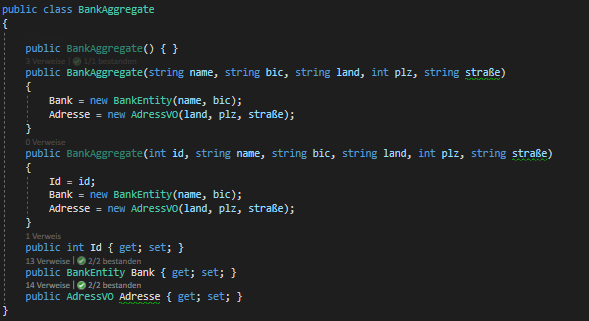
\includegraphics[width=10cm]{BankAggregate.png}}
    \caption{\label{bankAgg} BankAggregate}
\end{figure}
\subsection{Repositories}
Es wurden Repositories für User, Konto, Bank und Transaktion erstellt. Sie vermitteln zwischen der Domäne und dem Datenmodell. Innerhalb der Repositories werden Methoden zur Verfügung gestellt, 
um Aggregates aus dem Persistenzspeicher zu lesen, zu speichern oder zu löschen. Der Domain Code erhält dadurch Zugriff auf den persistenten Speicher, deren Implementierung wird der Domäne allerdings verborgen und ist somit flexibler. So wird eine Anti-Corruption-Layer zur Persistenzschicht gebildet.
Ein großer Vorteil von Repositories ist, dass zukünftig weitere Datenbanken einfach hinzugefügt oder ausgetauscht werden können, , ohne dass der Domain Code davon beeinflusst wird.
\newline Die wichtigsten Methoden eines Repository's sind diejenigen, die eine Aggregate Root Entity anhand ihrer Eigenschaften finden können. Dazu gehören beispielsweise die Funktionen eine Root Entity über ihre Id zu finden.
\newline Implementiert werden die Repositories in der Plugin-Schicht, da sie, wie bereits erwähnt, die Methoden zur Verfügung stellen um mit dem Persistenzspeicher zu arbeiten.
\newline In \ref{bankRepo} wird eines der erstellten Repositories gezeigt:
\begin{figure}[htbp]
    \centering
    \fbox{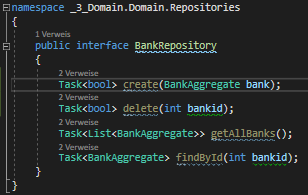
\includegraphics[width=10cm]{BankRepo.png}}
    \caption{\label{bankRepo} BankRepository}
\end{figure}
\subsection{Domain Services}
Domain Services dienen zum einen der Abbildung von komplexem Verhalten, das nicht eindeutig einer bestimmten Entity oder Value Object zugeordnet werden können und zum anderen als Definition eines \glqq Erfüllungs-Vertrages \grqq für externe Dienste, um zu verhindern, dass ein Domänenmodell nicht mit unnötiger \glqq accidental complexity \grqq belastet wird. Eine weitere wichtige Eigenschaft von Domain Services ist, dass sie selbst zustandslos sind.
\newline In diesem Projekt wurde beispielsweise ein Domain Service zur Überprüfung der Namens-, Email- und Passwortkonventionen erstellt. Dieser überprüft mit Hilfe einer Regular Expression bei Erstellung eines Benutzer, ob die übergebenen Parameter korrekt sind.
\newline In \ref{domServ} wird ein Ausschnitt des implementierten Domain Service gezeigt:
\begin{figure}[htbp]
    \centering
    \fbox{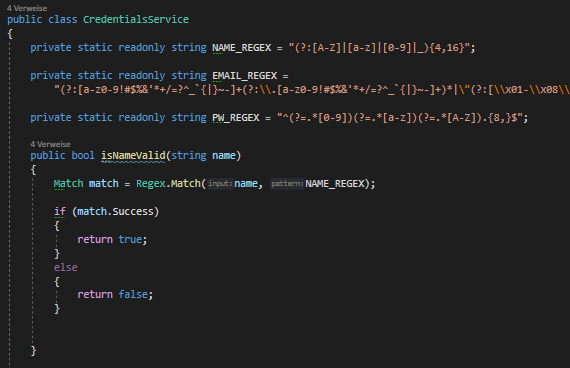
\includegraphics[width=10cm]{domServ.png}}
    \caption{\label{domServ} Ausschnitt aus CredentialsService}
\end{figure}


\chapter{Clean Architecture}
Die Architektur der WebApi wurde nach den Regeln der Clean Architecture geplant. Dabei gibt es 5 Schichten die implementiert werden können. Diese Schichten sind in \ref{cleanArchitecture} zu sehen:
\begin{figure}[htbp]
    \centering
    \fbox{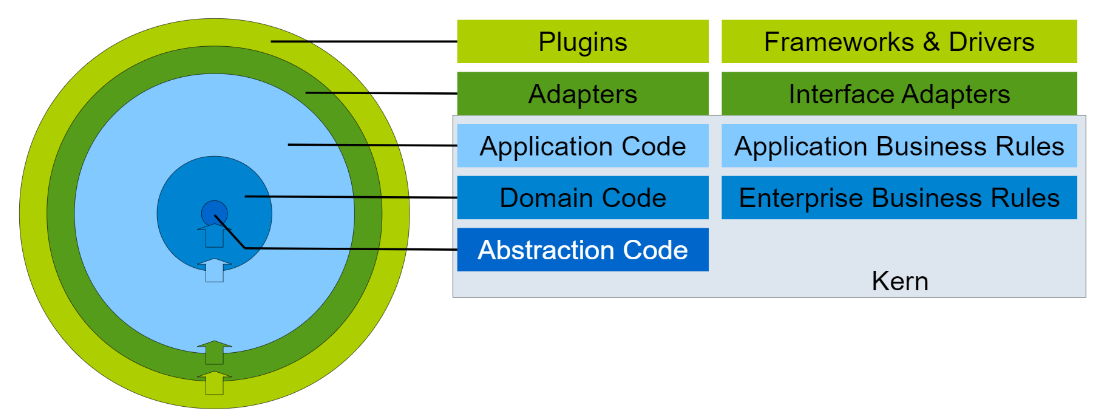
\includegraphics[width=10cm]{CleanArchitecture.png}}
    \caption{\label{cleanArchitecture} Schichten der Clean Architecture}
\end{figure}
Die Grundregeln der Clean Architecture besagen:
\begin{itemize}
    \item Der Anwendungs- und Domaincode ist frei von technischen Details
    \item Innere Schichten definieren Interfaces, äußere Schichten implementieren diese
    \item Sämtlicher Code kann eigenständig verändert werden
    \item Sämtlicher Code kann unabhängig von Infrastruktur kompiliert und ausgeführt werden
    \item Äußere Schichten koppeln sich an die inneren Schichten in richtung Zentrum
\end{itemize}
Hierbei ist die wichtigste aller Regeln, dass innere Schichten nicht von äußeren Schichten abhängen dürfen. Dadurch können äußere Schichten jederzeit ausgetauscht oder verädert werden, ohne dass die inneren Schichten etwas davon mitbekommen. 
Dies folgt auch dem Prinzip der Dependency Inversion.
\newline In diesem Projekt wurden 3 der 5 Schichten der Clean Architecture verwendet. Diese Schichten sind:
\begin{itemize}
    \item Plugin-Schicht
    \item Adapter-Schicht
    \item Domain-Schicht
\end{itemize}
Im Folgenden werden die verwendeten Schichten erklärt.
\section{Plugin-Schicht}
Die Plugin-Schicht ist die äußerste Schicht der Clean Architecture. Sie enthält die Klassen zum Starten der WebApi, stellt die Verbindung zur Datenbank her und führt Operationen auf der Datenbank aus.  
Außerdem liegen auf dieser Schicht die Controller, die die Anfragen entgegennehmen und Antworten zurück an den Client schicken.
\newline Sie implementiert die Repositories aus der Domain-Schicht und führt aufgrund dieser die Operationen auf der Datenbank aus. Die Adapter-Schicht wird verwendet , um die Ergebnisse aus der Datenbank umzumappen, 
damit sie an den Client zurückgeschickt werden können.  
\newline Die Plugin-Schicht ist die einzige Schicht, die externe Abhängigkeiten haben darf, da sie ganz außen liegt. In diesem Projekt ist dies beispielsweise 
durch die Abhängigkeit der Plugin-Schicht vom Entity Framework, das für die Datenbank-Operationen zuständig ist, zu sehen.
\section{Adapter-Schicht}
Die Adapter-Schicht konvertiert externe Formate so, dass die Applikation damit zurecht kommt und interne Formate so, dass externe Plugins damit zurecht kommen. Das Ziel dieser Struktur ist die Entkopplung von inneren und äußeren Schichten. Sie dient als Anti-Corruption Layer 
zwischen den Technischen Schichten und der Geschäftslogik.
\newline Da in diesem Programmentwurf mit einer InMemory-Datenbank, die innerhalb der Api läuft mit Hilfe der DbContext-Library und diese Einträge aufgrund der Entitäten der Anwendung baut, wird die Funktion externe Strukturen auf innere Strukturen abzubilden in der Adapter-Schicht nicht benötigt. 
Allerdings werden in der Adapter-Schicht in diesem Programmentwurf die interenen Strukturen wie Entitäten in Strukturen konvertiert, die an den Client weitergegeben werden können. Beispielsweise werden UserEntities in User-Objekte konvertiert, die nicht das Passwort des Benutzers enthalten, um eine Liste 
aller Benutzer in jedem Client darstellen zu können. Dadurch kann ein Benutzer alle anderen Benutzer sehen, um ihnen Geld zu überweisen, ohne dass der Client User-Objekte erhält, die das Passwort des Benutzers enthalten.
\section{Domain-Schicht}
In der Domain-Schicht befinden sich die Value Objects, Entities, Aggregates, Repositories und Domain Services. Die äußeren Schichten greifen auf diese Schicht zu, die Domain-Schicht kann aber auf keine andere Schicht zugreifen. Hier liegt die allgemeine Geschäftslogik. 
Dies hilft dabei zukünftig die Domain-Schicht auch in anderen Anwendungen verwenden zu können, wenn benötigt, da höchstens Abhängigkeiten von der Abstraction-Schicht bestehen, die sich nur sehr selten ändert. Die Repository-Interfaces, die in den äußeren Schichten implementiert werden, erlauben es der Domain-Schicht oder auch der Application-Schicht, wenn diese genutzt wird, auf die Datenbank zuzugreifen 
ohne von der Implementierung der Interfaces abhängig zu sein. Dadurch wird eine Inversion of Control erzeugt.
\newline Die Domain-Schicht in diesem Programmentwurf enthält alle der oben genannten Muster des Domain Driven Designs. 
\section{Weitere nicht implementierte Schichten}
\subsection{Application-Schicht}
In der Application-Schicht liegt die eigentliche anwendungsspezifische Geschäftslogik und die einzelnen Use Cases der Anwendung. Hier wird der Fluss der Daten von den Elementen der Domain-Schicht ausgehend und zu den Elementen führend gesteuert. 
Diese Schicht kann nur auf die Domain-Schicht zugreifen und Änderungen auf dieser Schicht beeinflussen die Domain-Schicht nicht. Sie funktioniert isoliert von Änderungen auf der Datenbank oder anderen Plugins, das bedeutet der genutzte Use Case weiß nicht, wer ihn aufgerufen hat oder auf 
welche Weise das Ergebnis präsentiert wird.
\newline Diese Schicht wurde in diesem Programmentwurf nicht explizit implementiert.
\subsection{Abstraction-Schicht}
Die Abstraction-Schicht enthält Domänen übergreifendes Wissen, wie Grundbausteine, die nicht domänenspezifisch sind, allgemeine Konzepte und Algorithmen oder nachgerüstete Libraries. Der Code auf dieser Schicht ändert sich selten bis nie und ist dadurch sehr stabil. Sie darf von keiner anderen Schicht abhängen, da 
sie nach dem Prinzip der Clean Architecture ganz innen liegt. In der Praxis muss diese Schicht häufig nicht explizit angelegt werden. Sie kann auch erst nachträglich eingebaut oder auch extrahiert werden. Genauere Beispiele für Code auf dieser Schicht sind beispielsweise Sortier-Algorithmen.
\newline Diese Schicht wurde in diesem Programmentwurf nicht explizit implementiert, da keine der zuvor genannten Bausteine oder Muster in dieser Anwendung verwendet werden.

\chapter{Programming Principles}
\section{SOLID}
SOLID setzt sich aus folgenden Prinzipien zusammen:
\begin{itemize}
    \item S: Single Responsibility Principle
    \item O: Open Closed Principle
    \item L: Liskov Substitution Principle
    \item I: Interface Segregation Principle
    \item D: Dependency Injection Principle
\end{itemize}
Für jedes dieser Prinzipien wird das vorkommen im Code dieses Programmentwurfs analysiert und begründet. Es kann jedoch durchaus vorkommen, dass eines dieser prinzipien nicht im Code auffindbar ist, da es nicht benötigt wurde.
\subsection{Single Responsibility Principle}
Das Single Responsibility Principle besagt, dass eine Klasse genau eine zuständigkeit haben sollte. Das bedeutet, dass jede Klasse eine klar definierte Aufgabe hat, wodurch eine niedrige Komplexität des Codes entsteht und eine niedrige Kopplung.
Durch die niedrige Komplexität des Codes lässt sich dieser auch einfacher warten und erweitern, da er besser verständlich ist.
\newline Angewendet wurde dieses Prinzip beispielsweise in der Adapter-Schicht. Hier wurde für das konvertieren jedes Objektes eine extra Klasse erstellt. Die Klasse \glqq UserAggregateToUserMapper \grqq ist nur dafür zuständig ein UserAggregate in ein User-Objekt umzuwandeln 
und nicht für Objekte andere Art zuständig. Nach diesem Prinzip gibt es für jedes Aggregat einen Mapper, der einem Aggregat entweder Eigenschaften, die der Client nicht benötigt oder erhalten sollte, entnimmt oder das Aggregat weniger komplex für den Client macht wie zum Beispiel der \glqq TransactionAggregateToTransactionMapper \grqq.
\subsection{Open Closed Principle}
Das Open Closed Principle macht eine Anwendung offen für Erweiterungen aber geschlossen für Änderungen. Das bedeutet, dass der Code nur durch Vererbung oder die Implementierung von interfaces erweitert wird. Dadurch muss bestehender Code nicht geändert werden. Um dies zu unterstützen, ist es von Vorteil viele Abstraktionen zu nutzen.
\newline In diesem Projekt wird dieses Prinzip vorallem in der Domain-Schicht sichtbar durch die Repository-Interfaces und die Domain Service-Interfaces. Es kann beispielsweise auf einfachste Weise neue Funktionen implementiert werden, indem ein neues Interface erstellt, das die neuen Funktionen nutzt und dieses Interface in der Plugin-Schicht implementiert wird. Daraufhin 
müssen keine Änderungen an anderen Klassen als dem erstellten Interface und der Klasse die dieses implementiert vorgenommen werden. 
\subsection{Liskov Substitution Principle}
Das Liskov Substitution Principle schränkt Ableitungsregeln stark ein, wodurch Invarianzen eingehalten werden. Dabei müssen abgeleitete Typen schwächere Vorbedingungen und stärkere Nachbedingungen besitzen, wodurch in der 
objektorientierten Programmierung eine \glqq verhält sich wie \grqq Beziehung entsteht. Wenn nun das Verhalten eines Basistypes bekannt ist, kann sich darauf verlassen werden, dass der abgeleitete Typ dieses Verhalten übernimmt.
\newline Dies ist beispielsweise bei der Implementierung der Repository-Interfaces zu sehen. Diese geben der Implementierung eine \glqq verhält sich wie \grqq Beziehung.
\subsection{Interface Segregation Principle}
Das Interface Segregation Principle besagt, dass Klassen, die ein Interface implementieren auch genau die Methoden des Interfaces implementieren, die sie benötigen und keine weiteren unnötigen Methoden. Dies wird umgesetzt, indem anstatt einem großen Interface, mehrere kleine Interfaces mit wenigen Funktionen genutzt.
Daraufhin werden genau die Interfaces in einer Klasse implementiert, die auch nur genau die Funktionen besitzen, die die klasse beötigt und keine weiteren Funktionen mitbringen, die nicht benötigt werden. 
\newline Da im Programmentwurf keine Interfaces bestehen, die in einer Klasse eine unnötige Methode implementieren, ist dieses Prinzip erfüllt.
\subsection{Dependency Inversion Principle}
Durch das Dependency Inversion Principle wird die klassische Struktur, in der High-Level Module von Low-Level-modulen abhängig sind umgekehrt. Dies geschieht, da Abstraktionen nicht von Details abhängig sein sollten. High-Level Module  
geben also die Regeln vor und Low-Level Module implementieren diese. Dadurch wird eine hohe Flexibilität der Software erreicht, da Low-level Module einfach ausgetauscht werden können, ohne dass High-Level Module ausgetauscht werden.
\newline Dieser Programmentwurf setzt dieses Prinzip durch die verwendete Schitenarchitektur der Clean Architecture um. Dabei werden die Repository- und Domain Service-Interfaces aus der High Level Domain-Schicht in den äußeren Low Level-Modulen implementiert und aufgerufen. 

\section{GRASP}
Grasp steht für General Responsibility Assignment Software Patterns. Diese beschreiben Basispattern, auf denen ein Entwurfsmuster aufbaut. Das Ziel dieses Prinzips ist es, die Low Representational Gap möglichst klein zu halten, was bedeutet, dass die Lücke zwischen dem 
gedachten Domänenmodell und der eigentichen Softwareimplementierung möglichst klein gehalten wird.
\subsection{Low Coupling}
Die Klassenkopplung ist ein Maß, das angibt, wie viele Klassen eine einzelne Klasse verwendet. Es wird versucht eine möglichst geringe Kopplung zu erreichen, wodurch eine geringere Abhängigkeit von Änderungen in anderen Teilen des Codes entsteht. 
Dies macht den Code außerdem einfacher zu testen und wiederverwendbar. Eine niedrige Kopplung macht den Code auch einfacher verständlich, da weniger Wissen über andere Klassen benötigt wird. Eine lose Kopplung macht Komponenten austauschbarer.
\newline Kopplung entsteht beispielsweise durch das Halten von Attributen, deren Typ eine andere Klasse ist, durch das Aufrufen bzw. Besitzen von Methoden mit Referenz auf eine andere Klasse oder wenn Interfaces verwendet werden.
Eine Klasse kann an konkrete oder abstrakte Datentypen gekoppelt sein, an Threads, die gemeinsame Sperren besitzen oder auch an Resourcen, die gemeinsame Dateien nutzen. Dabei ist jedoch die Kopplung an stabilere Komponenten weniger problematisch.
\newline In Visual Studio kann standardmäßig die Klassenkopplung eines Projektes berechnet werden. Dabei kann für jede klasse des projektes die klassenkopplung begutachtet werden.
\newline In diesem Programmentwurf wird durch die inversion of Control erreicht, dass die Kopplung von Klassen hauptsächlich an stabilere komponenten besteht. Die meisten Klassen sind hauptsächlich von inneren Klassen, also von stabileren Komponenten abhängig. Diese 
Komponenten sind stabiler, da sie seltener geändert werden, als die Klassen auf äußereren Schichten. Ein Beispiel hierfür ist, dass die Mapper auf der Adapter-Schicht hauptsächlich von Klassen der Domain-Schicht abhängig sind.
\subsection{High Cohesion}
Die Kohäsion ist ein Maß, das für den zusammenhalt einer Klasse steht. Es wird die semantische Nähe der Elemente einer Klasse beschrieben. 
\newline Ein wichtiges Prinzip ist das \glqq High Cohesion \& Low Coupling \grqq -Prinzip. Es ist das Fundament für einen idealen Code, da dieses Prinzip zu einem einfacheren und verständlicherem Design des Codes führt. 
Dieses Prinzip ist jedoch schwer automatisiert testbar, weshalb es hauptsächlich das menschliche Ermessen benötigt, um zu entscheiden ob es gut umgesetzt ist oder nicht.
\newline Der Zusammenhalt der Klassen in diesem Projekt ist gut. Dies wird vorallem in den Entities oder Value Objects in der Domain-Schicht klar, da hier zu sehen ist, dass diese nur Eigenschaften besitzen, die semantisch zu ihnen passen.
Ein Beispiel wäre das \glqq AdressVO \grqq . Es besitzt nur Eigenschaften, die zu einer Adresse passen, wie das Land, die Postleitzahl und die Straße, in der sich das Objekt befindet. 
Ein weiteres Beispiel ist die \glqq UserEntity \grqq -Klasse. Diese besitzt nur Eigenschaften, die semantisch zu einem angelegten benutzer passen. Dies sind die Email-Adresse, der Name des Benutzer und das Passwort, das benltigt wird um sich mit diesem benutzer anzumelden.
\subsection{Information Expert}
Bei diesem Prinzip geht es um die allgemeine Zuweisung einer Zuständigkeit zu einem Projekt. Am einfachsten ist dies umzusetzen, indem einem Objekt, das eine bestimmte Information besitzt, auch die Zuständigkeit für diese Information überreicht wird. 
Dafür muss allerdings im Designmodell eine passende Klasse existieren. Sollte dies nicht der Fall sein , wird im Domänenmodell eine passende Repräsentation gesucht und dafür eine passende Klasse im Designmodell erstellt. Dieses Objekt ist dann zuständig für die Informationen, die es besitzt. Dadurch entsteht eine Kapselung 
von Informationen und leichteren Klassen.
\newline In diesem programmentwurf ist dieses Prinzip in den Aggregaten sichtbar. Diese übernehmen die Verantwortung über die enthaltenen Entities und deren Informationen bzw. über die 
enthaltenen Value Objects. Ein Beispiel hierfür wäre das \glqq BankAggregate \grqq . Dieses übernimmt die Zuständigkeit über die Informationen des \glqq AdressVO \grqq und die \glqq BankEntity \grqq .
\subsection{Creator}
Das Creator-Prinzip legt fest, wer für die Erzeugung eines Objektes zuständig ist. Ein Objekt kommt als Creator eines anderen Objektes in Frage, wenn es eine Beziehung zu jedem erstellten Objekt gibt. 
Dadurch wird die Kopplung der Komponenten verringert. 
\newline In diesem Programmentwurf sind ein Beispiel für dieses Prinzip die Mapper auf der Adapter-Schicht. Sie konvertieren Objekte und erzeugen dadurch ein neues Objekt einer anderen Klassen. Hier gibt es für jedes Objekt einen eigenen Mapper, 
weshalb die Beziehung zwischen den Objekten und dem Mapper hergestellt ist. Dadurch wird auch die kopplung der Klassen verringert.
\subsection{Indirection}
Das Indirection-Prinzip besagt, dass ein System oder die Teile eines Systems voneinander entkoppelt werden. Dies ist allerdings mit viel Aufwand verbunden, bietet jedoch einen höheren Freiheitsgrad als die Nutzung von Vererbung oder Polymorphismus.
\newline In diesem Programmentwurf wurde dies beispielsweise durch die Repository-Schnittstellen erreicht. Dieses wurden so designed, dass sie genau ihrem Anwendungszweck angepasst sind und somit eine höhere Flexibilität erreichen.
\subsection{Polymorphism}
Polymorphismus ist ein grundlegendes Prinzip der objektorientierten Programmierung. Dabei erhalten Methoden, je anch Typ eine andere Implementierung. Dadurch werden Fallunterscheidungen vermieden, wie If-Else bzw. Switch-Statements. 
Es werden dafür abstrakte Klassen oder Interfaces als Basistypen genutzt. Polymorphismus macht eine Anwendung einfacher erweiterbar, da die bestehende Struktur nicht verändert werden muss. Außerdem können Frameworks einfacher extrahiert werden. 
\newline Im Programmentwurf wird dies beispielsweise in der \glqq UserRepositoryImpl \grqq deutlich. Dieses implementiert das zugehörige Repository-Interface und fügt noch spezifische Funktionen hinzu. Das Interface 
kann somit auch in weiteren Klassen implementiert werden, wo es benötigt wird und daraufhin weitere spezifische Funktionen innerhalb der Klasse hizufügen.
\subsection{Controller}
Das Controller-Prinzip besagt, dass in diesen Klassen einkommende Benutzereingaben verarbeitet werden. Sie dienen der koordination zwischen Benutzeroberfläche und Businesslogik. Dabei werden 
die Benutzereingaben an andere Objekte delegiert, denn im Controller befindet sich keinerlei Businesslogik. 
\newline Unterschieden werden Controller in System Controller, der für alle Aktionen des Systems zuständig ist und nur für kleine Anwendungen praktikabel ist und in Use Case Controller. Use Case Controller 
werden für jeden einzelnen Use Case implementiert.
\newline In diesem Programmentwurf wurden die Use Case Controller genutzt, die auf der Plugin-Schicht implementiert sind. Folgende Use Case Controller wurden implementiert:
\begin{itemize}
    \item UserController
    \item KontoController
    \item TransactionController
    \item BankController
\end{itemize}
Diese Controller nehmen einkommende Benutzereingaben an und delegieren sie. Daraufhin erhalten sie ein Ergebnis und senden die zurück an den Client, der die Anfrage geschickt hat.
\subsection{Pure Fabrication}
Dieses Prinzip besagt, dass eine Klasse keinen Bezug zur Problemdomäne besitzt, wodurch eine Trennung von Technologie und Problemdomäne, sowie eine Kapselung von Algorithmen entsteht. Dadurch wird erreicht, 
dass Softwareteile auch außerhalb der Domäne wiederverwendet werden können. Außerdem wird durch die kapselung von speziellen Funktionalitäten das High Cohesion-Prinzip begünstigt. Es sollte jedoch möglichst wenig vorkommen.
\newline In diesem Programmentwurf wird dieses Prinzip einmal verwendet durch die Klassen, die eine Email an den Benutzer versendet, die die Transaktionen eines Kontos enthält. Diese Klassen können abgekapselt vom Rest der 
Problemdomäne und können leicht wiederverwendet werden. Diese klassen befinden sich auf der Domain-Schicht im Ordner \glqq Others \grqq .
\subsection{Protected Variations}
Dieses Prinzip besagt, dass die Software durch die Kapselung verschiedener Implementierungen hinter einer einheitlichen Schnittstelle vor Variationen gesichert wird. Der Einfluss der Variabilität einer einzelnen Komponente soll nicht das 
Gesamtsystem betreffen. Gute Schutzmöglichkeiten hierfür sind Polymorphie und Delegation. Weitere Möglichkeiten sind Stylesheets im Webumfeld oder Spezifikationen von Schnittstellen.
\newline Im Programmentwurf wird dies durch die Nutzung der Repository-Interfaces, die abgekapselt implementiert werden können, für neue Datenbanken.

\section{DRY}
DRY steht für \glqq Don't repeat yourself \grqq . Dieses Prinzip kann beispielsweise auf Datenbankschemata, Testpläne, Buildsysteme oder Dokumentationen angewendet werden. Es besagt, dass nur eine Quelle der 
Wahrheit bestehen darf und alle anderen Quellen von dieser abgeleitet werden. Dies ist vergleichabr mit den Normalformen bei RDBMS.
\newline Die Auswirkungen einer Modifikation eines Teils haben eine definierte Reichweite. Dabei sind jedoch keine unbeteiligten Teile betroffen und alle relevanten Teile ändern sich automatisch.
\newline Es gibt drei Arten von Duplikationen, die durch das DRY-Prinzip behandelt werden:
\subsubsection{Imposed Duplication}
Imposed Duplications sind auferlegte Duplikationen. Dabei glaubt der Entwickler die Duplikation ist unumgänglich.
\subsubsection{Inadverted Duplication}
Inadverted Duplications sind versehentliche Duplikationen, die der Entwickler nicht bemerkt.
\subsubsection{Impatient Duplication}
Impatient Duplications sind ungeduldige Duplikationen, wobei der Entwickler zu faul ist, um diese zu beseitigen.
\subsection{Anwendung des DRY-Prinzips}
Bie der Erstellung dieses Programmentwurfs wurde von Anfang an darauf geachtet, dass kein duplizierter Code erstellt wird. Es soll eher bestehender Code an verschiedenen Stellen wiederverwendet werden. Duplizierter Code kann zu folgenden Problemen führen:
\begin{itemize}
    \item Bei Änderungen kann es zu Inkonsistenzen kommen, die möglicherweise ein Sicherheits-Risiko darstellen. Es müssen nämlich daraufhin alle Stellen geändert werden, die den duplizierten Code enthalten, wobei es vorkommen kann, dass eine Stelle vergessen wird.
    \item Duplizierter Code macht den Programmcode länger und unübersichtlicher.
    \item Duplizierter Code führt zu duplizierten Bugs
\end{itemize}
Im Programmentwurf wurde beispielsweise der \glqq CredentialsService \grqq verwendet, der dafür sorgt, dass Name, Email und Password den Konventionen entsprechen. Dieser Service wird an einer Stelle implementiert und kann daraufhin von mehreren Stellen aufgerufen werden, 
um Duplikationen zu verhindern. Dadurch sind auch Änderungen am Service an allen Stellen automatishc korrekt. Außerdem gibt es die Mapper der Adapter-Schicht, die an mehreren Stellen aufgerufen werden, um Konvertierungen auszuführen. Änderungen an den Datenstrukturen müssen nur innerhalb der 
Mapper geändert werden, damit sie überall korrekt sind.
\chapter{Entwurfsmuster}
\section{Singleton-Entwurfsmuster}
Das Singleton-Entwurfsmuster besagt, dass von einer Klasse systemweit nur ein Objekt existiert. Dies wird sichergestellt, indem innerhalb der Klasse, in der das Entwurfsmuster angewendet wird, 
eine getInstance-Methode existiert, die anstatt des Konstruktors von externen Klassen aufgerufen wird. Weiterhin existiert innerhalb der Klasse ein Attribut vom Typ dieser Klasse, das als Instanz dient. 
Die getInstance-Methode prüft, ob das instance-Attribut bereits existiert oder nicht. Sollte das instance-Attribut noch nicht existieren wird der Konstruktor aufgerufen und das erstellte Objekt 
in das instance-Attribut gespeichert und daraufhin zurückgegeben. Sollte das instance-Attribut existieren, wird das Attribut zurückgegeben.
\section{Einsatz}
Im Programmentwurf wurde dieses Entwurfsmuster beispielsweise in den Mappern genutzt. Diese werden nur einmal instanziiert und können daraufhin durch die getInstance-Methode von überall 
aufgerufen werden. So muss nicht jedesmal, wenn ein Mapper benötigt wird, eine neue Instanz des Mappers erzeugt werden, wodurch auch die Systemresourcen geschont werden. Außerdem wird eine Instanz auch nur dann angelegt, wenn sie benötigt wird.
\newpage
\section{Vorher-Nachher-Vergleich}
\begin{figure}[htbp]
    \centering
    \fbox{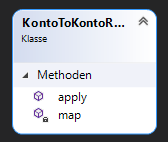
\includegraphics[width=5cm]{KtoKMapperVorher.png}}
    \caption{\label{singletonVorher} Singleton Vorher}
\end{figure}
\begin{figure}[htbp]
    \centering
    \fbox{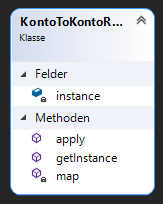
\includegraphics[width=5cm]{KtoKMapperNachher.png}}
    \caption{\label{singletonNachher} Singleton Nachher}
\end{figure}

\chapter{Refactoring}
\section{Code Smell 1 - Lange Methode}
Der erste Code Smell, der identifiziert wurde, ist langer übersichtlicher Code, der dafür genutzt wurde, um Transaktionen in einer Mail aufzulisten und an den eingeloggten Benutzer zu versenden. 
Diese Methode ist die \glqq getTransactionsAsMail \grqq -Methode, die sich in der \glqq TransactionRepositoryImpl \grqq -Klasse befindet.
In dieser Methode werden zum einen alle Transaktionen für ein Konto abgerufen und zum anderen ein Mail-Objekt aufgrund der abgefragten Transaktionen erstellt. Es wurde, um die Übersichtlichkeit zu 
verbessern, die Funktion, die das Mail-Objekt erstellt, in eine neue Methode extrahiert. In \ref{codeSmell1} ist die unübersichtliche Methode zu sehen. In \ref{codeSmell1Nachher} ist die Methode zu sehen nach dem Refactoring.
\begin{figure}[htbp]
    \centering
    \fbox{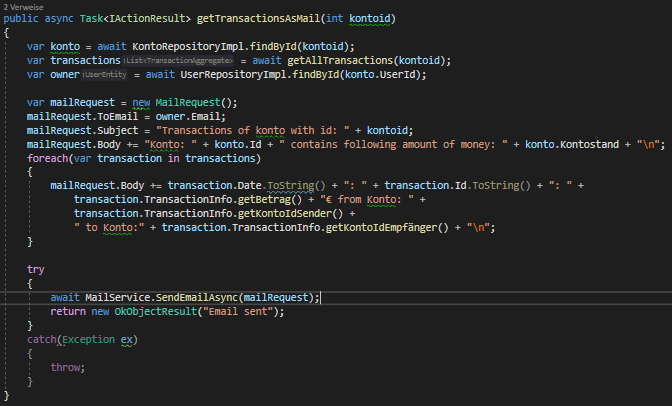
\includegraphics[width=10cm]{CodeSmell1Vorher.png}}
    \caption{\label{codeSmell1} Long Method}
\end{figure}
\begin{figure}[htbp]
    \centering
    \fbox{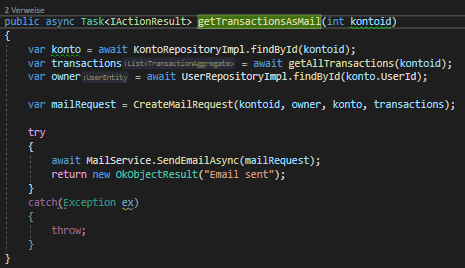
\includegraphics[width=10cm]{CodeSmell1Nachher.png}}
    \caption{\label{codeSmell1Nachher} Long Method Refactored}
\end{figure}
\section{Code Smell 2 - Duplikate im Code}
Der zweite Code Smell, der identifiziert wurde, ist ein Duplikat im Code. Es wurde zwar versucht nach dem DRY-Prinzip zu arbeiten, dies wurde jedoch nicht hundertprozentig umgesetzt. Später lies sich beispielsweise in der \glqq UserController \grqq -Klasse 
ein Duplikat finden, in welchem eine Liste an UserEntities in eine Liste von User-Objekten durch einen den Mapper konvertiert wurde. Diese Funktion wurde in mehreren Methoden dieser Klasse verwendet. 
\newline Um das Duplikat zu verhindern, wurde diese Funktion in eine neue Methode innerhalb des Mappers ausgelagert, durch welche nun eine Liste an UserEntities in eine Liste an User-Objekten umgewandelt wird. 
Diese Methode wird von mehreren Stellen aufgerufen. In \ref{codeSmell2Vorher} wird der Code, der dupliziert vorkam, in einer der Methoden gezeigt.
\begin{figure}[htbp]
    \centering
    \fbox{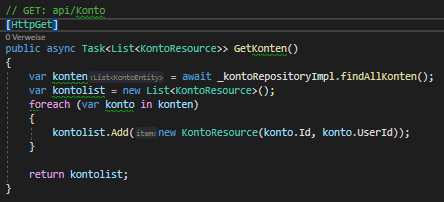
\includegraphics[width=10cm]{CodeSmell2Vorher.png}}
    \caption{\label{codeSmell2Vorher} Duplicate Code}
\end{figure}
\begin{figure}[htbp]
    \centering
    \fbox{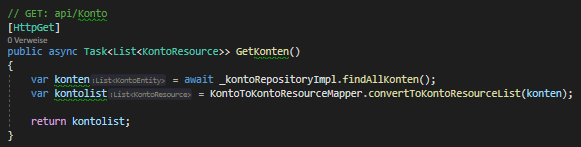
\includegraphics[width=10cm]{CodeSmell2Nachher.png}}
    \caption{\label{codeSmell2Nachher} Duplicate Code Refactored}
\end{figure}
In \ref{codeSmell2Nachher} wird gezeigt, wie die Funktion ausgelagert wurde und durch den Mapper aufgerufen wird. Diese Funktion wird noch an weiteren Stellen innerhalb des Controllers aufgerufen.
\chapter{Unit Tests}
In diesem Programmentwurf wurden 11 Unit Tests erstellt.
\section{Mocking}
Im Projet \glqq Programmentwurf\_BankingAp\_Mock\_Tests \grqq wurde ein Unit Test erstellt, der die Datenbank mockt. Dafür wurde \glqq IBankingContext \grqq gemockt und ein 
Unit Test erstellt, der die Methode \glqq findById \grqq testet.
\section{Unit Tests}
Weiterhin wurde für die Methoden der verschiedenen Mapper-Klassen Unit tests erstellt, um deren Funktion zu testen.
\section{Ausführen der Tests}
Um die Tests auszuführen, wird in Visual Studio der Test-Explorer geöffnet und von dort aus die Tests ausgeführt.
\newline Um in Visual Studio Code die Tests auszuführen wird in das jeweilige Projekt navigiert und über die Terminal-Konsole der Befehl \glqq dotnet test \grqq eingegeben.
\include{7_kapitel}
\include{8_kapitel}
\pagenumbering{roman}
\setcounter{page}{\thesavepage}
% Ab hier beginnt der Anhang
\appendix
%%\addcontentsline{toc}{chapter}{Anhang}

%%\addcontentsline{toc}{chapter}{Index}
%%\printindex

\addcontentsline{toc}{chapter}{Literaturverzeichnis}

% Haben Sie das "biblatex"-Paket nicht installiert, benutzen Sie folgendes:
% Ohne das "biblatex"-Paket (s. bericht.sty) produziert folgendes
% "deutsche" Zitate in Literaturverzeichnissen gemaß der Norm DIN 1505,
% Teil 2 vom Jan. 1984.
% Die Zitatmarken werden alphabetisch nach Verfassern
% sortiert und sind durch abgekürzte Verfasserbuchstaben plus
% Erscheinungsjahr in eckigen Klammern gekennzeichnet.

% \bibliographystyle{alphadin}
% \bibliography{bericht}

%%%%%%%%%%%%%%%%%%%%%%%%%%%%%%%%%%%%%%%5
% BIBLATEX
% Benutzt man das "biblatex"-Paket, muß man folgendes schreiben:
\def\refname{Literaturverzeichnis}
\printbibliography
%%%%%%%%%%%%%%%%%%%%%%%%%%%%%%%%%%%%%%%5


% 30 mtime=1458147391.399548382
30 atime=1458147391.401548365
30 ctime=1458147391.399548382


% \newpage
% \addcontentsline{toc}{chapter}{Liste der ToDo's}
% \listoftodos[Liste der ToDo's]


\end{document}
